\documentclass[tikz, border=2mm]{standalone}
\usepackage{bm}

\begin{document}
    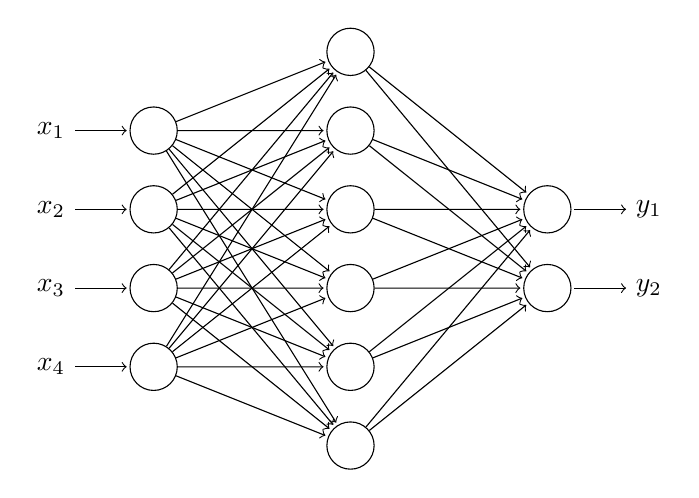
\begin{tikzpicture}
        % Number of input neurons
        \newcommand{\inputnum}{4}
        % Number of neurons in the hidden layer
        \newcommand{\hiddennum}{6}
        % Number of output neurons
        \newcommand{\outputnum}{2}
        % Input Layer
        \foreach \i in {1,...,\inputnum} {
            \node[
                circle,
                minimum size = 6mm,
                draw=black
            ] (Input-\i) at (0,-\i) {};
        }
        % Hidden Layer
        \foreach \i in {1,...,\hiddennum} {
            \node[
                circle,
                minimum size = 6mm,
                draw=black,
                yshift=(\hiddennum-\inputnum)*5 mm
            ] (Hidden-\i) at (2.5,-\i) {};
        }
        % Output Layer
        \foreach \i in {1,...,\outputnum} {
            \node[
                circle,
                minimum size = 6mm,
                draw=black,
                yshift=(\outputnum-\inputnum)*5 mm
            ] (Output-\i) at (5,-\i) {};
        }
        % Connect neurons In-Hidden
        \foreach \i in {1,...,\inputnum} {
            \foreach \j in {1,...,\hiddennum} {
                \draw[->, shorten >=1pt] (Input-\i) -- (Hidden-\j);
            }
        }
        % Connect neurons Hidden-Out
        \foreach \i in {1,...,\hiddennum} {
            \foreach \j in {1,...,\outputnum} {
                \draw[->, shorten >=1pt] (Hidden-\i) -- (Output-\j);
            }
        }
        % Inputs
        \foreach \i in {1,...,\inputnum} {
            \draw[<-, shorten <=1pt] (Input-\i) -- ++(-1,0)
            node[left]{$x_{\i}$};
        }
        % Outputs
        \foreach \i in {1,...,\outputnum} {
            \draw[->, shorten <=1pt] (Output-\i) -- ++(1,0)
            node[right]{$y_{\i}$};
        }
    \end{tikzpicture}
\end{document}
